% Created 2021-04-20 Tue 19:43
% Intended LaTeX compiler: pdflatex

\documentclass[english]{article}
\usepackage[T1, T2A]{fontenc}
\usepackage[lutf8]{luainputenc}
\usepackage[english, russian]{babel}
\usepackage{minted}
\usepackage{graphicx}
\usepackage{longtable}
\usepackage{hyperref}
\usepackage{xcolor}
\usepackage{natbib}
\usepackage{amssymb}
\usepackage{stmaryrd}
\usepackage{amsmath}
\usepackage{caption}
\usepackage{mathtools}
\usepackage{amsthm}
\usepackage{tikz}
\usepackage{grffile}
\usepackage{extarrows}
\usepackage{wrapfig}
\usepackage{algorithm}
\usepackage{algorithmic}
\usepackage{lipsum}
\usepackage{rotating}
\usepackage{placeins}
\usepackage[normalem]{ulem}
\usepackage{amsmath}
\usepackage{textcomp}
\usepackage{capt-of}

\usepackage{geometry}
\geometry{a4paper,left=2.5cm,top=2cm,right=2.5cm,bottom=2cm,marginparsep=7pt, marginparwidth=.6in}
 \usepackage{hyperref}
 \hypersetup{
     colorlinks=true,
     linkcolor=blue,
     filecolor=orange,
     citecolor=black,      
     urlcolor=blue,
     }

\date{}
\title{}
\hypersetup{
 pdfauthor={},
 pdftitle={},
 pdfkeywords={},
 pdfsubject={},
 pdfcreator={Emacs 28.0.50 (Org mode 9.4.4)}, 
 pdflang={English}}
\begin{document}

\begin{titlepage}
    \begin{center}
        \large\textbf{Федеральное государственное автономное образовательное учреждение высшего образования ``Национальный исследовательский университет ИТМО``} \\
        \vspace{0.5cm}
        Факультет информационных технологий и программирования \\
        \vspace{0.5cm}
        Направление ``Прикладная математика и информатика`` \\
        \vspace{3cm}
        Отчет к лабораторной работе №2 \\
        \vspace{0.5cm}
        \textbf{Методы многомерной оптимизации}
    \end{center}
    \vfill
    \begin{flushright}
        \large
        Выполнили студенты группы М3237 \\
        \vspace{0.5cm}
        Ярошевский Илья \\
        Аникина Вероника \\
    Крюков Александр
    \end{flushright}
    \vspace{3cm}
    \begin{center}
        Санкт-Петербург 2021
    \end{center}
\end{titlepage}

\section{Цели работы}

\begin{enumerate}
    \item Реализовать алгоритмы
    \begin{itemize}
        \item Метод градиентного спуска
        \item Метод наискорейшего спуска
        \item Метод сопряженных градиентов
    \end{itemize}
    \item Проанализировать траектории методов для некоторых квадратичных функций
    \item Исследовать количество итераций в зависимости от размерности пространства и числа обусловленности
\end{enumerate}
\section{Ход работы}

Во всех тестах начальное приближение --- вектор размерности
пространства из единиц, точность \(\varepsilon\) = 0.001, ограничение на
количество итераций --- 10000 \\
Исходный код: \href{https://github.com/iliayar/MethOpt}{https://github.com/iliayar/MethOpt}
\subsection{Количество итераций}
На графиках:
\begin{itemize}
    \item Горизонтиаль --- число обусловленности
    \item Вертикаль --- количество итераций
\end{itemize}
Для исследования количества итераций использовались случайно сгенерированные функции вида \(f(x) = \frac{1}{2} A x^2 + b x + c\) с парамаметрами:
\begin{itemize}
    \item \(A\) --- диагональная матрица с заданным числом обусловленности.
    \item \(b\) --- вектор размерности пространства из единиц.
    \item \(c = 0\)
\end{itemize}
Для каждого числа обусловленности производились тесты на двух функциях. На графиках представленны средние значения количества итераций из этих двух тестов.
\subsubsection{Метод градиентного спуска}
\begin{center}
    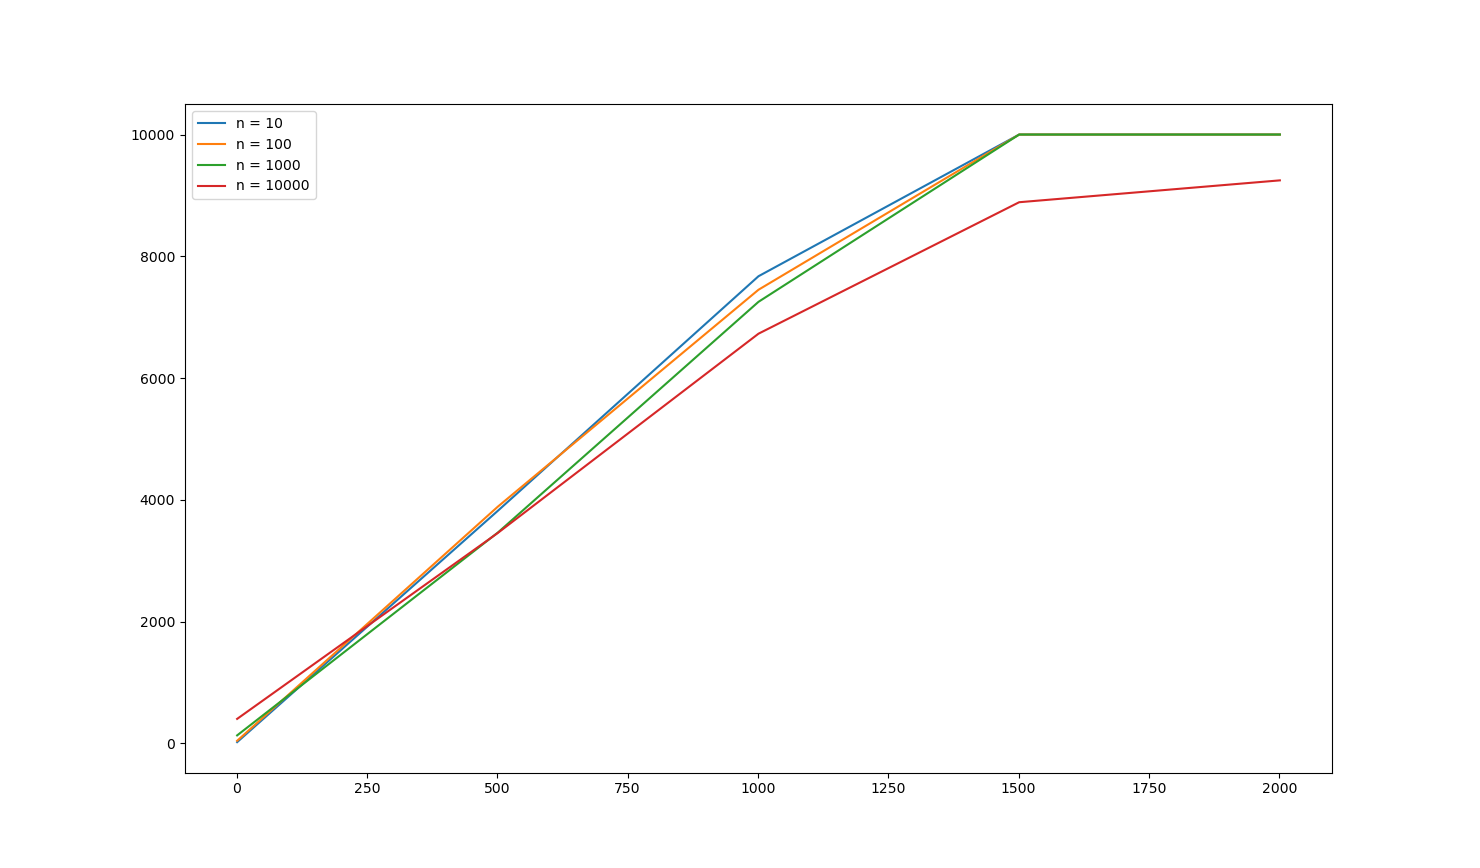
\includegraphics[scale=0.4]{plots/gradient_descent_1.png}
\end{center} 
Видно, что количество итераций не
зависит от размерности пространства \(n\), но линейно зависит от числа
обусловленности \(k\)

\subsubsection{Метод наискорейшего спуска}

\begin{center}
    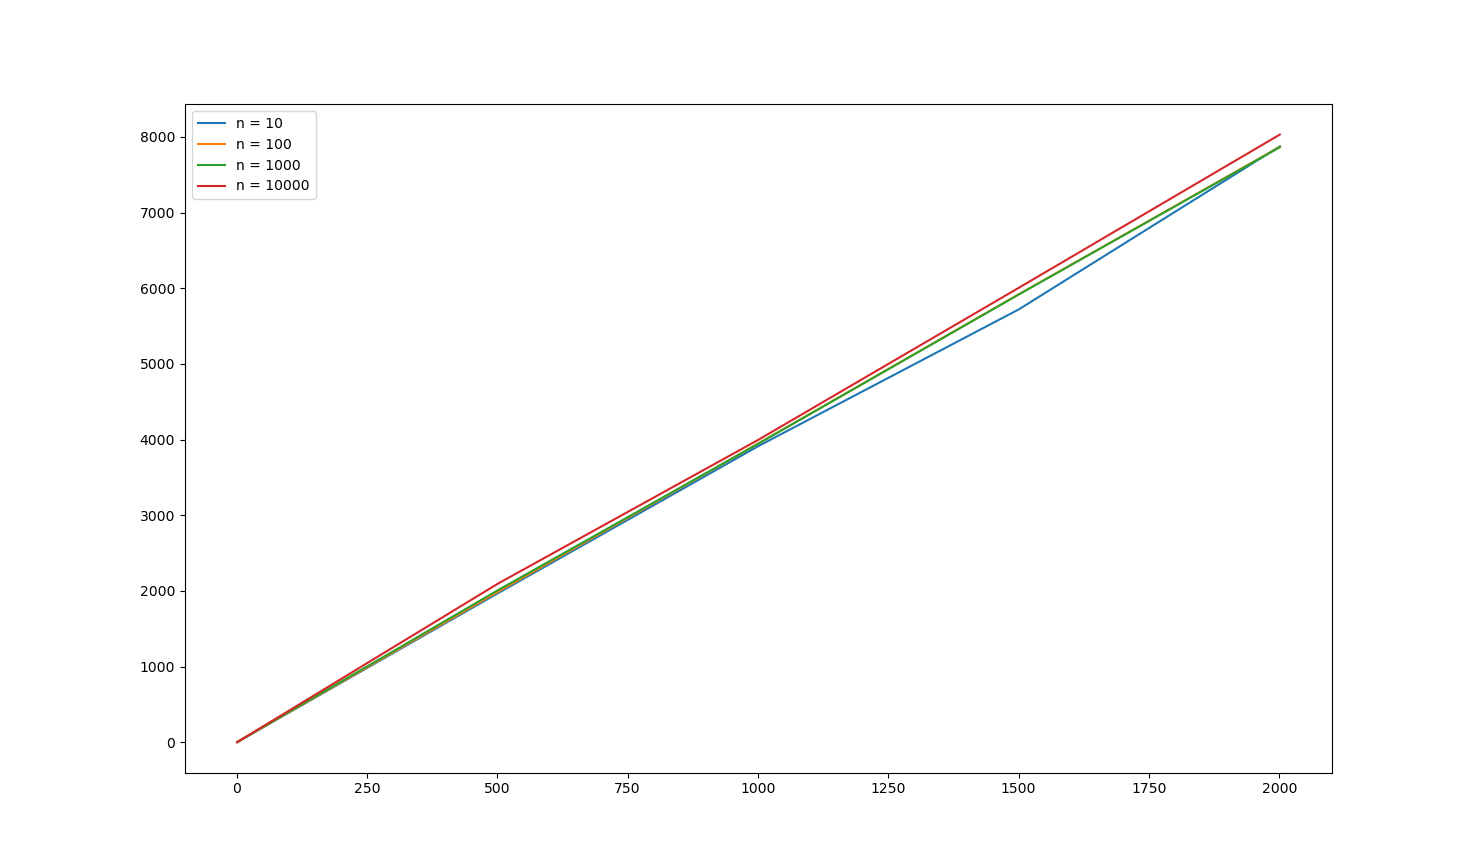
\includegraphics[scale=0.4]{plots/steepest_gradient_1.png}
\end{center} 
Так же как и в методе градиентного
спуска можно видеть линейную зависимость количества итераций от числа
обусловленности. Количество итераций так же не зависит от размерности
пространства.

\subsubsection{Метод сопряженный градиентов}
\begin{center}
    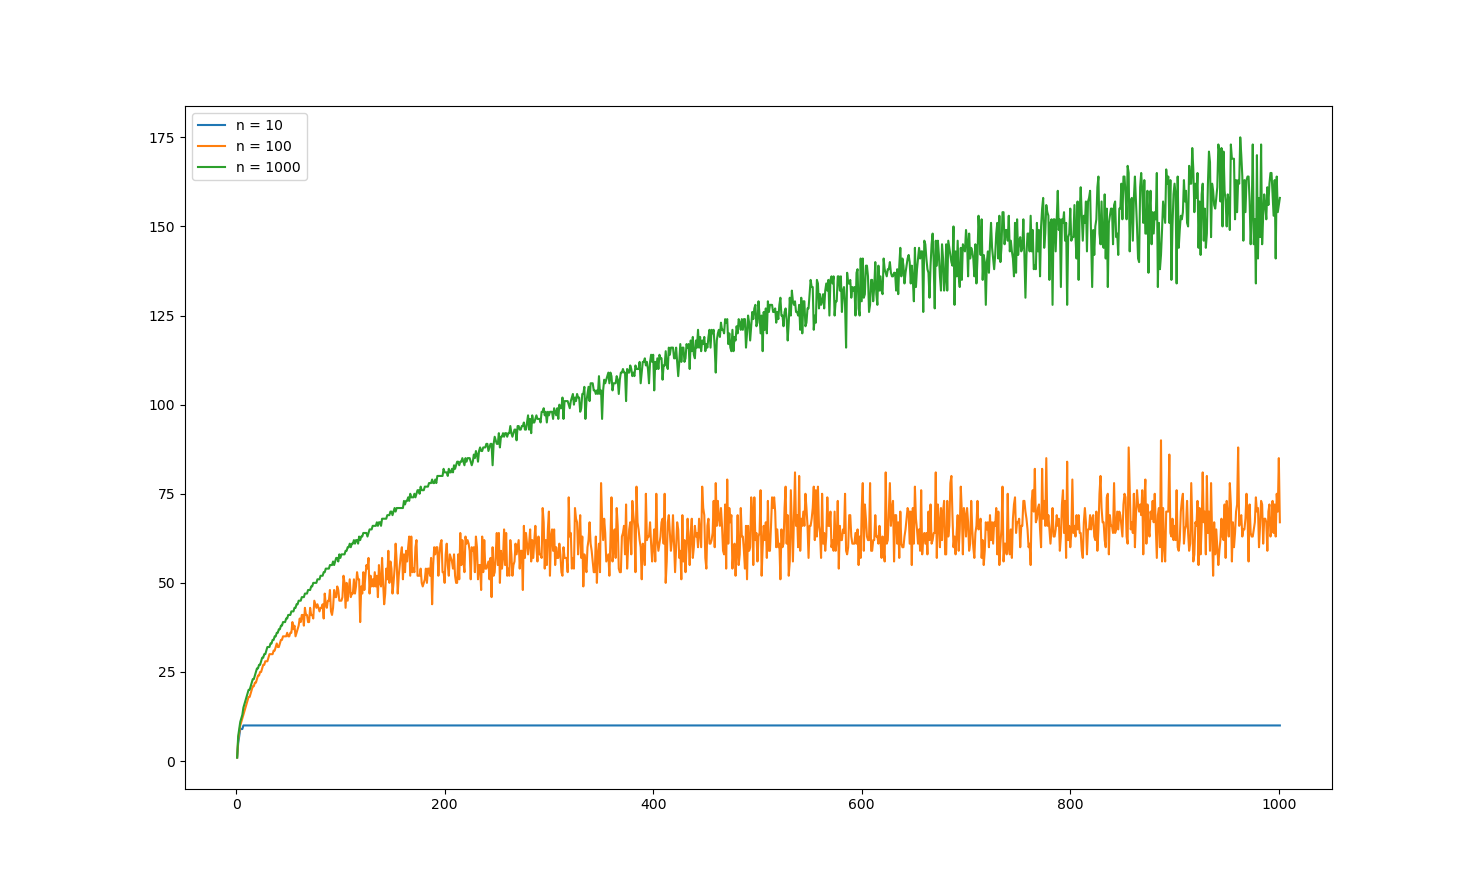
\includegraphics[scale=0.4]{plots/conjugate_gradient_1.png}
\end{center}
Видно что количество итераций нелинейно зависит от числа
обусловленности. Так же можно отметить, что количество итераций всегда
будет не больше размерности пространства.

\subsection{Траектории}
\[ f_1(x) = \frac{1}{2}\begin{pmatrix}
100 & -1 \\
-1 & 1
\end{pmatrix} x^2 + \begin{pmatrix} -10 & 0 \end{pmatrix}x\]
Все методы находят минимум функции \(f_1^* = -0.50505\) в точке \(x^* = (0.101011\ 0.1011)\)
\[ f_2(x) = \frac{1}{2}\begin{pmatrix}
3 & -1 \\
-1 & 2
\end{pmatrix} x^2 + \begin{pmatrix} -5 & 2 \end{pmatrix}x\]
Все методы находят минимум функции \(f_2^* = -4.2\) в точке \(x^* = (1.6\ -0.2)\)
\[ f_3(x) = \frac{1}{2}\begin{pmatrix}
1 & -1 \\
-1 & 2
\end{pmatrix} x^2 + \begin{pmatrix} -10 & 2 \end{pmatrix}x\]
Все методы находят минимум функции \(f_3^* = -82\) в точке \(x^* = (18\ 8)\) \\

\subsubsection{Метод градиентного спуска}
\begin{center}
    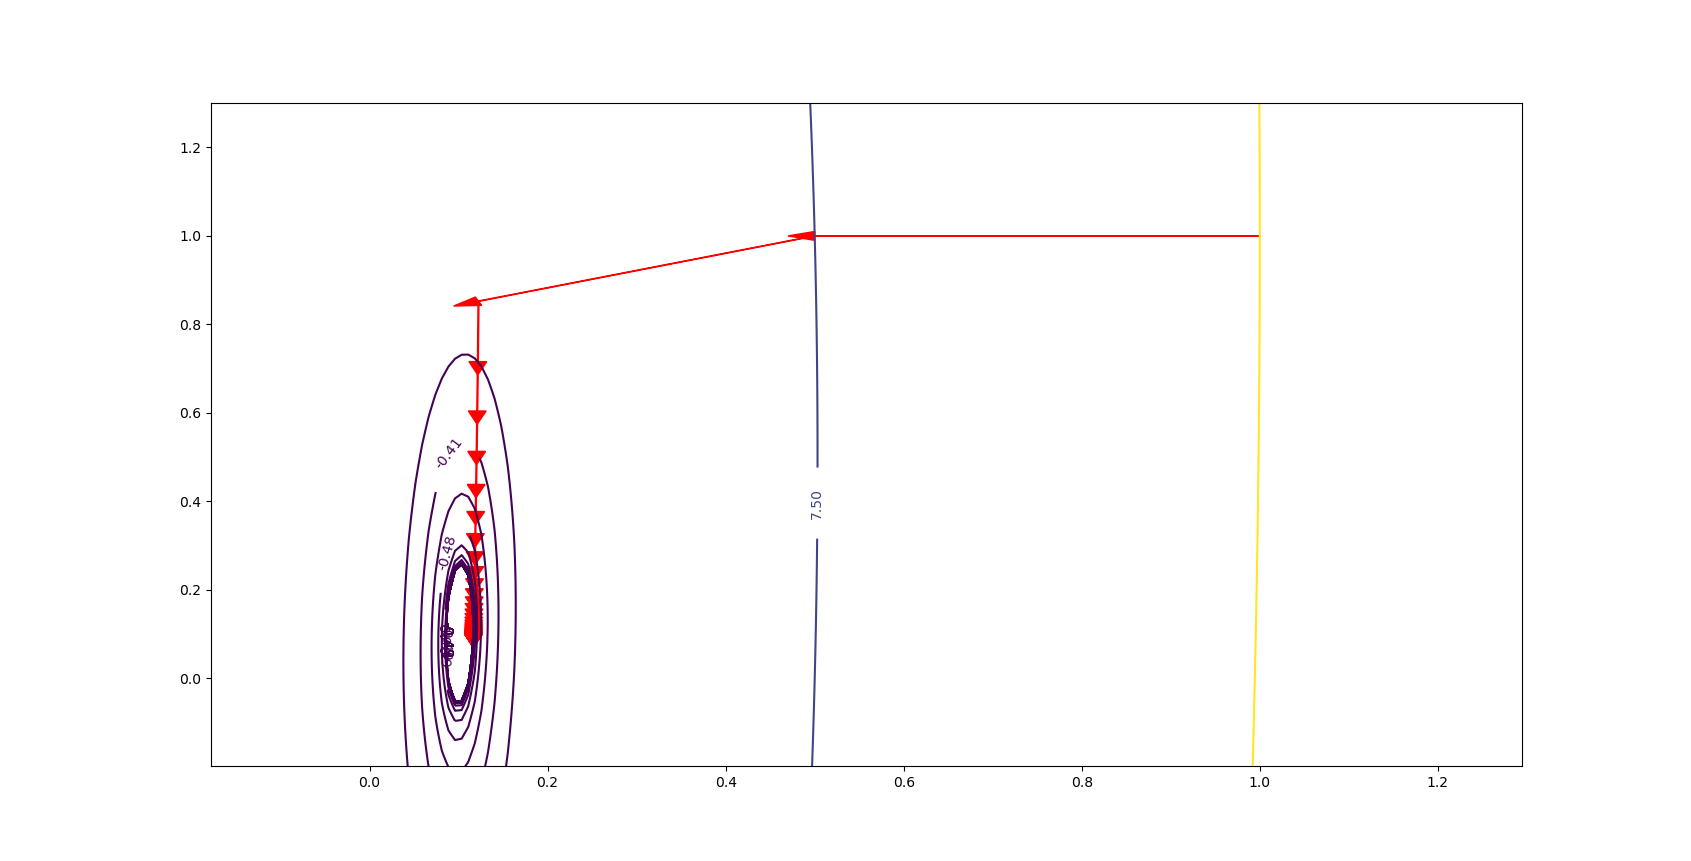
\includegraphics[scale=0.3]{plots/traectories/gradient_descent_1.png}
    \captionof{figure}{Траектория метода на функции \(f_1\)}
\end{center}
\begin{center}
    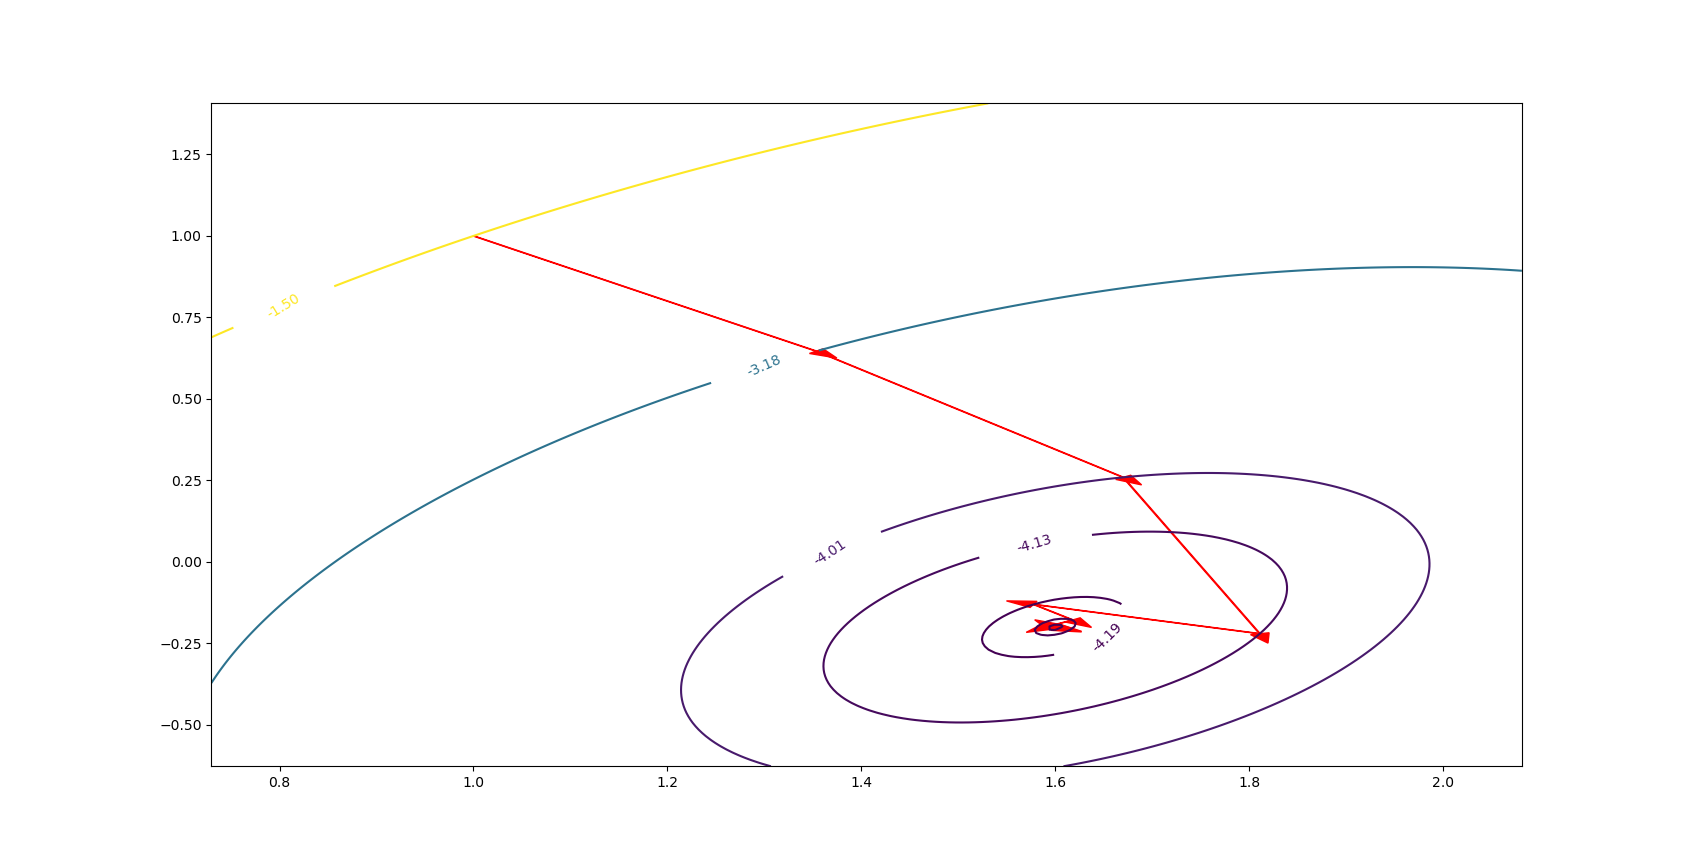
\includegraphics[scale=0.3]{plots/traectories/gradient_descent_2.png}
    \captionof{figure}{Траектория метода на функции \(f_2\)}
\end{center}
\begin{center}
    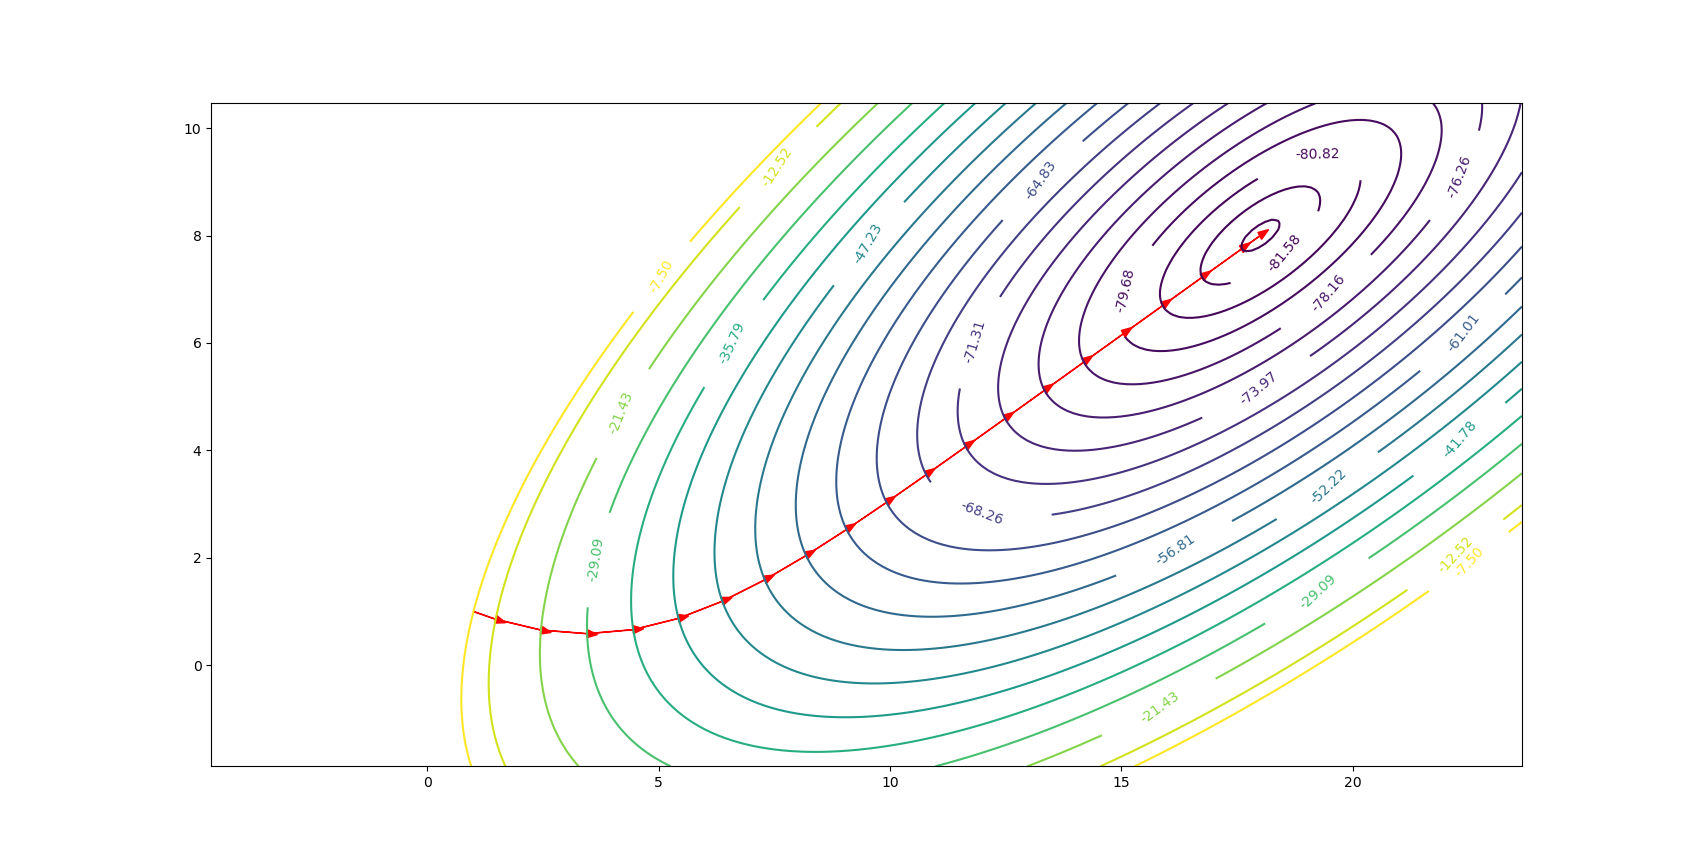
\includegraphics[scale=0.3]{plots/traectories/gradient_descent_3.png}
    \captionof{figure}{Траектория метода на функции \(f_3\)}
\end{center}

При запуске на \(f_1\) методу потребовалось гораздо больше шагов
(\(\approx\) 800) дла нахождения минимума в отличии от функций \(f_2\)
(\(\approx\) 10 шагов) и \(f_1\) (\(\approx\) 40 шагов), так как число
обусловленности матрицы \(A\) функции \(f_1\) достаточно велико \(\mu
= 100\).
\subsubsection{Метод наискорейшего спуска}
\begin{center}
    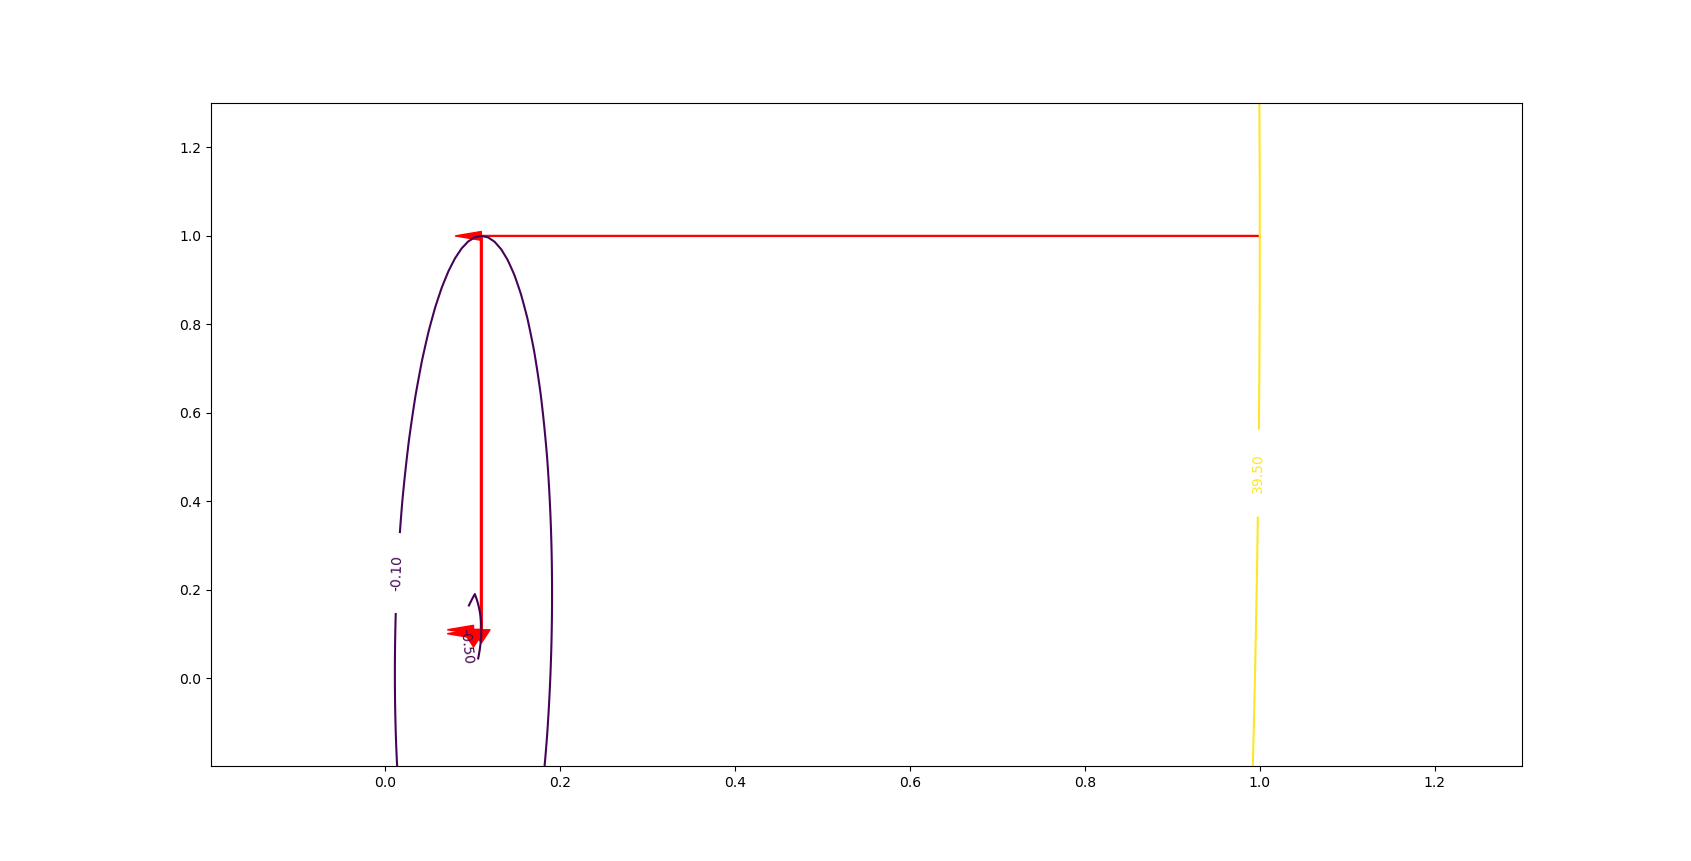
\includegraphics[scale=0.3]{plots/traectories/steepest_descent_1.png}
    \captionof{figure}{Траектория метода на функции \(f_1\)}
\end{center}
\begin{center}
    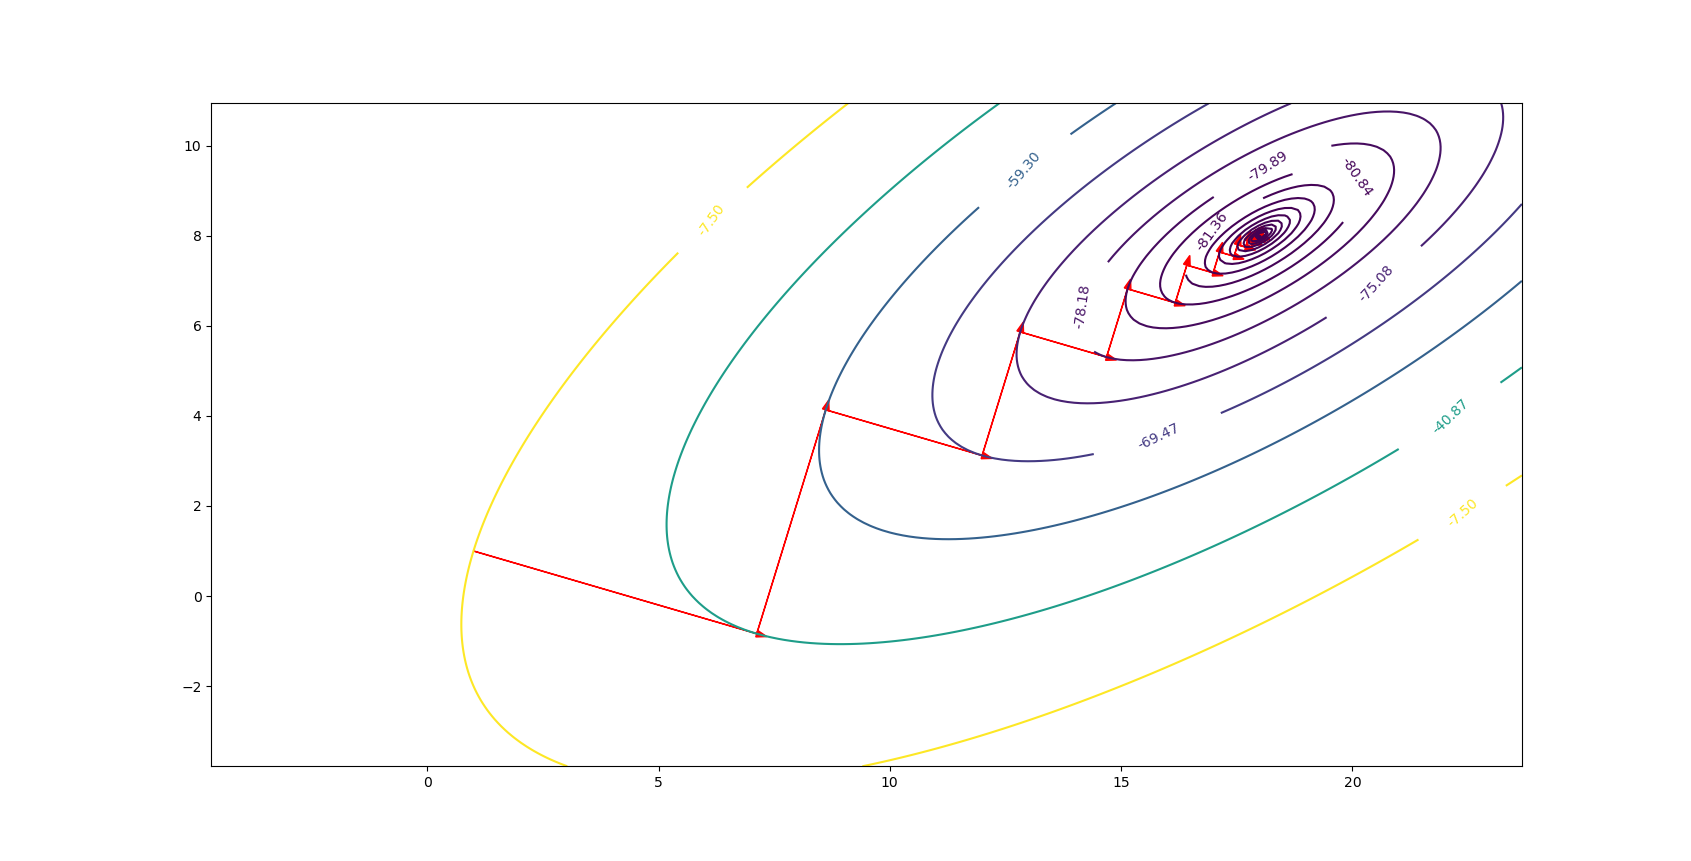
\includegraphics[scale=0.3]{plots/traectories/steepest_descent_3.png}
    \captionof{figure}{Траектория метода на функции \(f_3\)}
\end{center}

Не смотря на высокое число обусловленности функции \(f_1\), метод
потребовалось 5 шагов для нахождения минимума. Но в то же время на
функции \(f_3\) потребовалось всего 2 шага.

\subsubsection{Метод сопряженных градиентов}
\begin{center}
    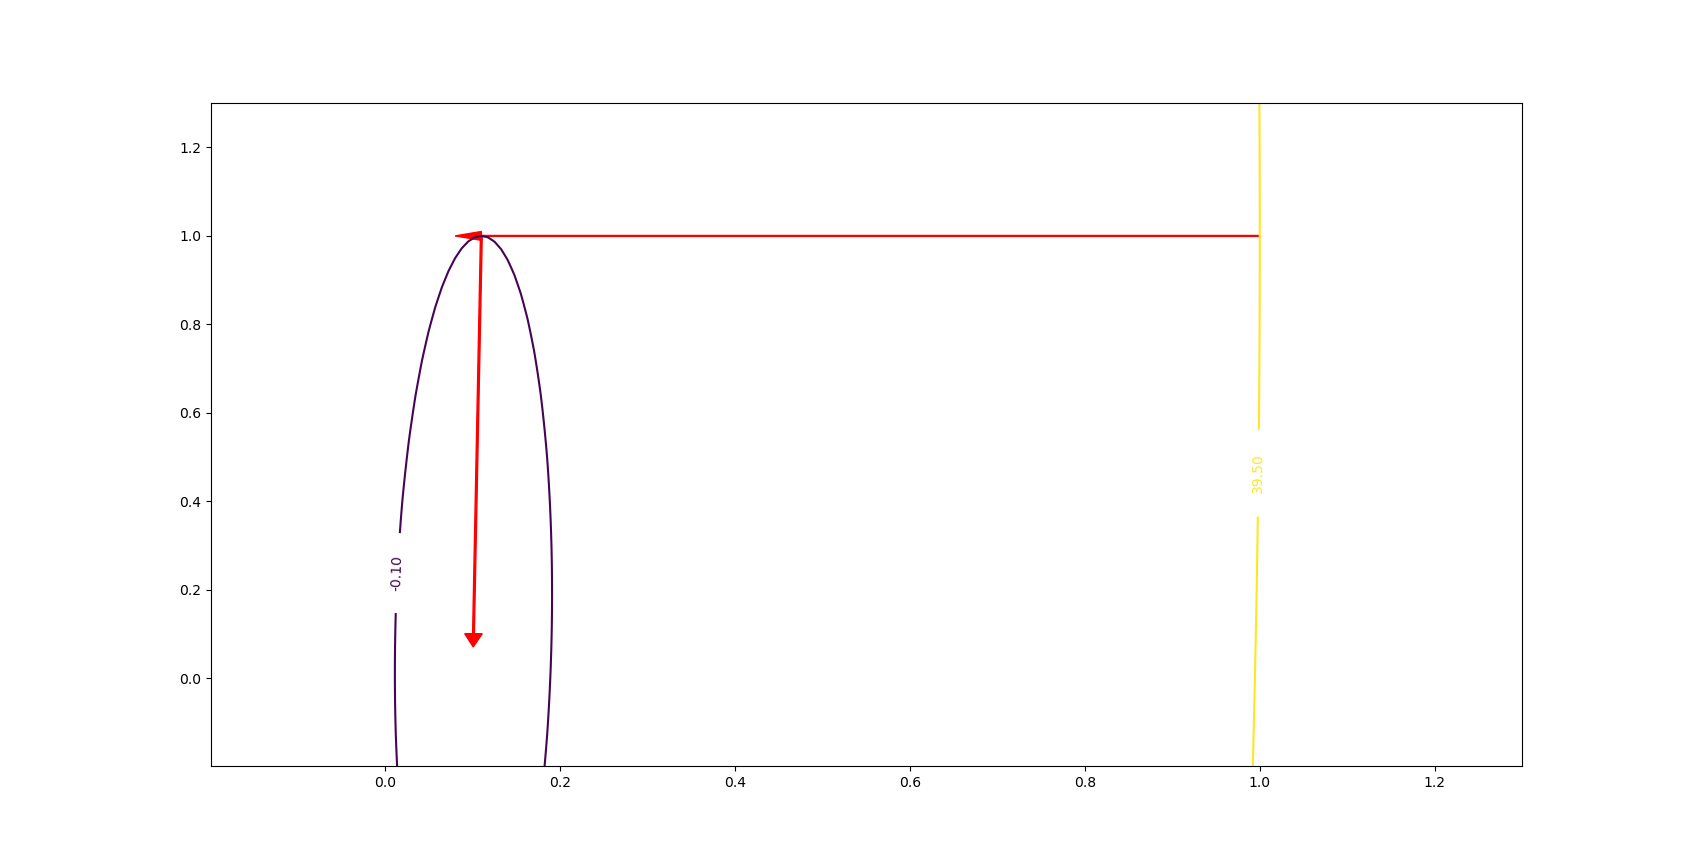
\includegraphics[scale=0.3]{plots/traectories/conjugate_gradient_1.png}
    \captionof{figure}{Траектория метода на функции \(f_1\)}
\end{center}
\begin{center}
    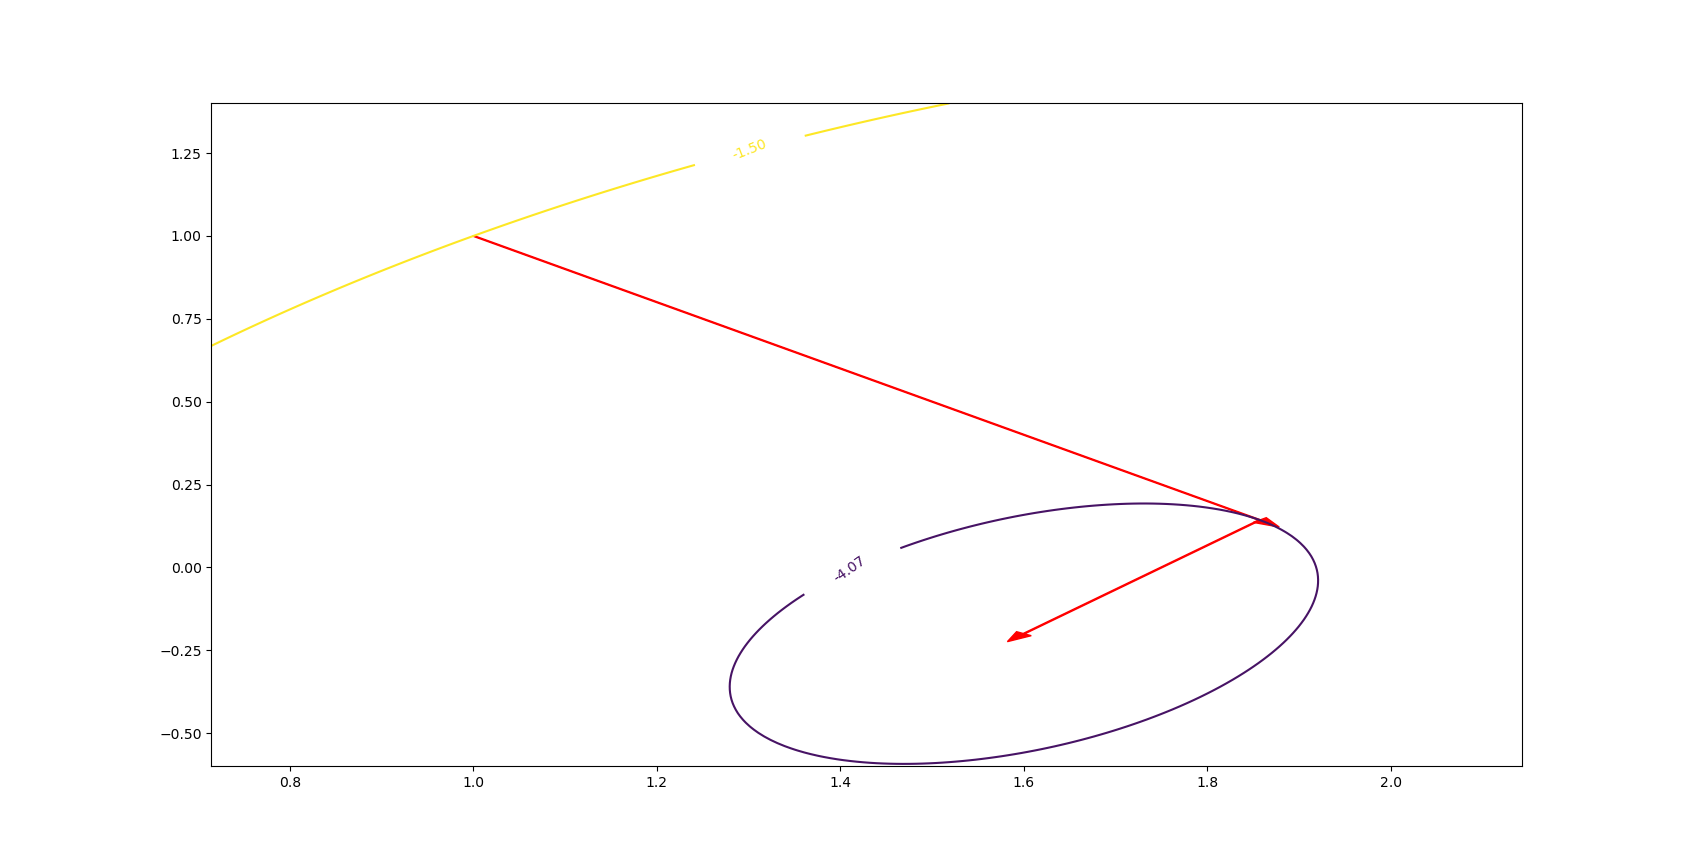
\includegraphics[scale=0.3]{plots/traectories/conjugate_gradient_2.png}
    \captionof{figure}{Траектория метода на функции \(f_2\)}
\end{center}
\[ f_0(x) = \frac{1}{2}\begin{pmatrix}2 & -1 \\ -1 & 2\end{pmatrix}x^2 \quad x^0 = (1, 1) \]
\begin{center}
    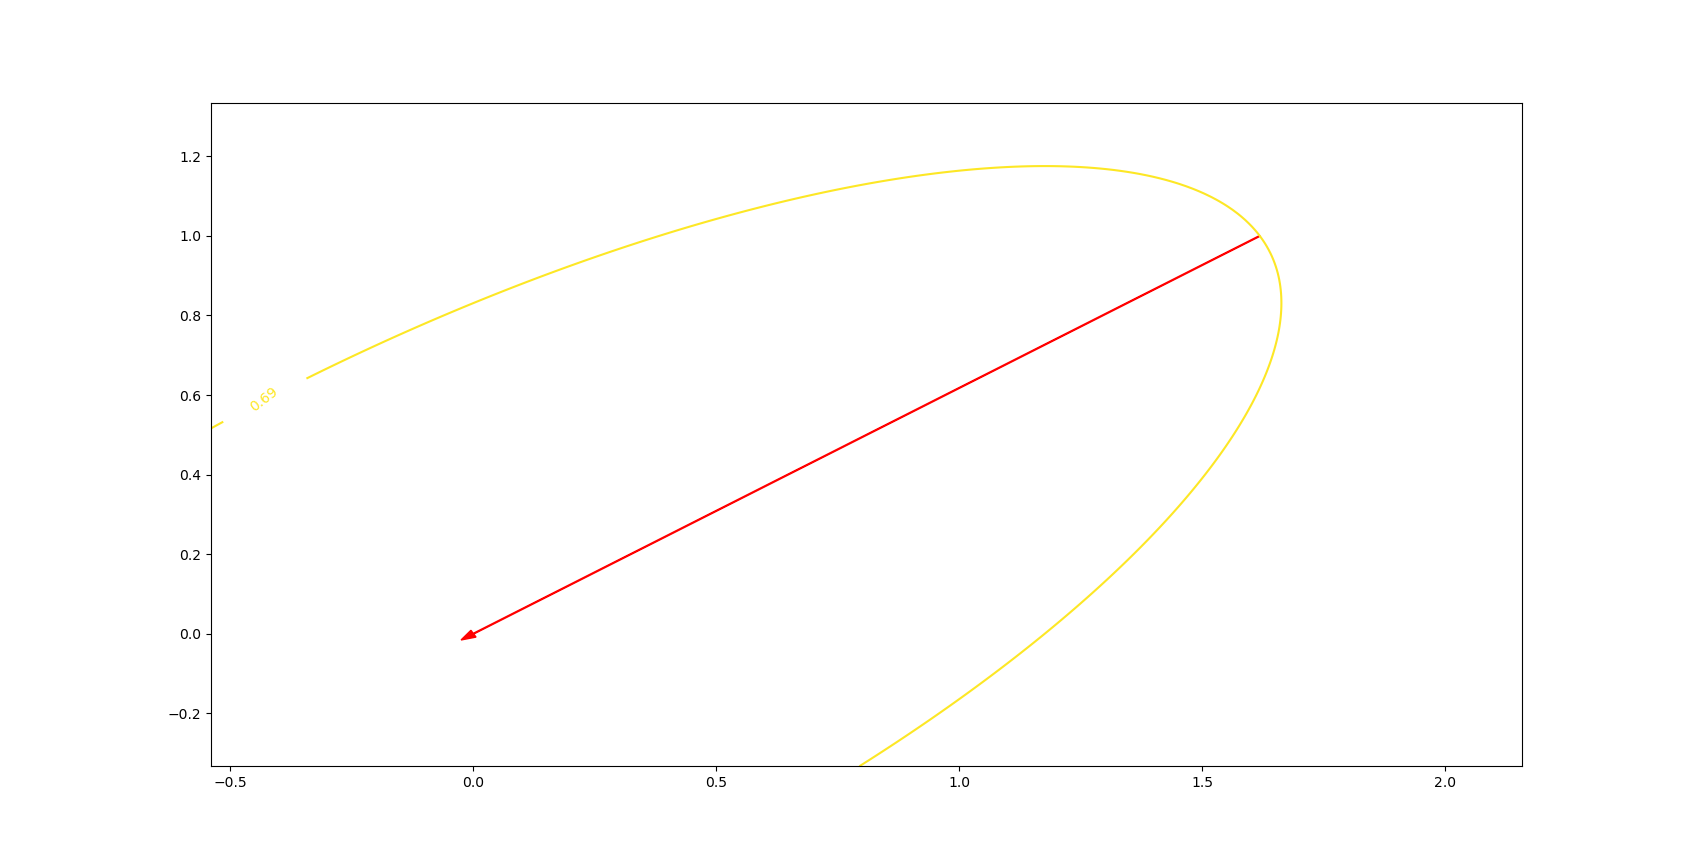
\includegraphics[scale=0.3]{plots/traectories/conjugate_gradient_3.png}
    \captionof{figure}{Траектория метода на функции \(f_0\) с начальным приближением \(x_0\)}
\end{center}

Данный метод находит точку минимума на заданных функциях за два или три шага. В случае 3, когда начальное приближение равно собственному вектору матрицы \(A\) и \(b = (0, 0)\), метод находит точку минимума за один шаг. Это свойство также будет верно и для метода сопряженных градиентов. 

\end{document}
